% Full datapath (itmn_m2/src/top/Mamba_Top.v): two clusters, their memories, mirrored writes, barrier, GN exchange.
\documentclass[tikz,border=4pt]{standalone}
% Shared style of the RTL diagrams. Build one with: tectonic fig_x.tex
\usepackage{tikz}
\usetikzlibrary{arrows.meta,positioning,fit,calc,backgrounds,shapes.geometric}
\usepackage[T1]{fontenc}
\usepackage{lmodern}
% opaque background, so the SVGs stay readable on dark pages
\tikzset{every picture/.append style={show background rectangle,
         background rectangle/.style={fill=white, draw=none}, inner frame sep=2pt}}
\definecolor{inkA}{HTML}{0B0B0B}
\definecolor{inkB}{HTML}{52514E}
\definecolor{rule}{HTML}{C3C2B7}
\definecolor{fillA}{HTML}{F0EFEC}
\definecolor{fillPE}{HTML}{CDE2FB}
\definecolor{fillRow}{HTML}{FBE0D3}
\definecolor{fillMem}{HTML}{E5F4EC}
\definecolor{fillCtl}{HTML}{FDF0C8}
\definecolor{fillReg}{HTML}{F6C9A8}
\definecolor{ctlink}{HTML}{8A6A00}
\tikzset{
  blk/.style={draw=inkB, line width=0.5pt, rounded corners=1.5pt, align=center, font=\scriptsize, inner sep=2pt},
  pe/.style={blk, fill=fillPE},
  row/.style={blk, fill=fillRow},
  mem/.style={blk, fill=fillMem},
  ctl/.style={blk, fill=fillCtl},
  plain/.style={blk, fill=white},
  grp/.style={draw=rule, line width=0.6pt, rounded corners=3pt, inner sep=4pt},
  dgrp/.style={draw=inkB, dashed, line width=0.5pt, rounded corners=3pt, inner sep=4pt},
  arr/.style={-{Stealth[length=3pt]}, line width=0.5pt, draw=inkB},
  darr/.style={{Stealth[length=3pt]}-{Stealth[length=3pt]}, line width=0.5pt, draw=inkB},
  carr/.style={-{Stealth[length=2.5pt]}, line width=0.4pt, draw=ctlink, densely dashed},
  lbl/.style={font=\scriptsize, text=inkB, align=center},
  tlbl/.style={font=\tiny, text=inkB, align=center},
  clbl/.style={font=\tiny, text=ctlink, align=center},
  opc/.style={circle, draw=inkB, fill=white, line width=0.5pt, minimum size=0.42cm, inner sep=0pt, font=\scriptsize},
  mux/.style={trapezium, trapezium stretches=true, trapezium angle=70, draw=inkB, fill=fillA, line width=0.5pt, minimum height=0.38cm,
              inner sep=1pt, font=\tiny, shape border rotate=180},
  regbar/.style={draw=inkB, fill=fillReg, line width=0.5pt, minimum height=0.16cm, inner sep=0pt},
}
% bus width mark: \bw{coordinate}{width}
\newcommand{\bw}[2]{\draw[line width=0.4pt, draw=inkB] ($(#1)+(-0.06,-0.06)$) -- ($(#1)+(0.06,0.06)$)
  node[tlbl, anchor=west, inner sep=1pt] {#2};}

\tikzset{dma/.style={-{Stealth[length=3pt]}, line width=0.5pt, draw=inkB!70, dashed},
         mm/.style={mem, minimum width=1.1cm, minimum height=0.85cm, font=\tiny, inner sep=1pt}}
% \clusterbody{suffix}{outer column x}{inner column x}{centre x}
\newcommand{\clusterbody}[4]{
  \node[ctl, minimum width=2.8cm] (fsm#1) at (#3,10.4) {controller FSM\\stages, job table, addresses};
  \node[ctl, minimum width=2.6cm] (opr#1) at (#2,9.0) {operand registers};
  \node[plain, minimum width=2.6cm] (lut#1) at (#3,9.0) {LUT\_Bank: SiLU, softplus,\\exp (16 lanes), rsqrt};
  \node[pe, minimum width=2.6cm, minimum height=1.2cm] (mcl#1) at (#2,7.45) {M\_Cluster\\16 PE lanes, 32 DSP\\H\_RegFile, URAM};
  \node[plain, minimum width=2.6cm] (red#1) at (#3,7.45) {Reduce16Wide\\RN $\Sigma x^2$, 45 bit};
  \node[row, minimum width=2.6cm] (cha#1) at (#2,5.8) {C$\cdot$h row\\16 mult., tree A};
  \node[row, minimum width=2.6cm] (gtb#1) at (#3,5.8) {gate row\\16 mult., tree B};
  \node[plain, minimum width=4.6cm] (cmb#1) at (#4,4.35) {split-K combine: $\mathrm{sat16}((acc + aux) \gg 11)$, + bias};
  \draw[carr] (fsm#1) -| ($(opr#1.north)!0.45!(fsm#1.south |- opr#1.north)$);
  \draw[carr] (fsm#1) -- (lut#1);
  \draw[arr] (opr#1) -- (mcl#1);
  \draw[arr] (lut#1) -- (opr#1);
  \draw[arr] (mcl#1) -- (red#1);
  \draw[arr] (mcl#1) -- (cha#1) node[tlbl, pos=0.5, right] {$h_\mathrm{new}$};
  \draw[arr] (cha#1) -- (gtb#1) node[tlbl, pos=0.5, above] {$y_\mathrm{ssm}$};
  \draw[arr] (cha#1) -- (cha#1 |- cmb#1.north) node[tlbl, pos=0.5, right] {aux A};
  \draw[arr] (gtb#1) -- (gtb#1 |- cmb#1.north) node[tlbl, pos=0.5, right] {aux B};
}
\begin{document}
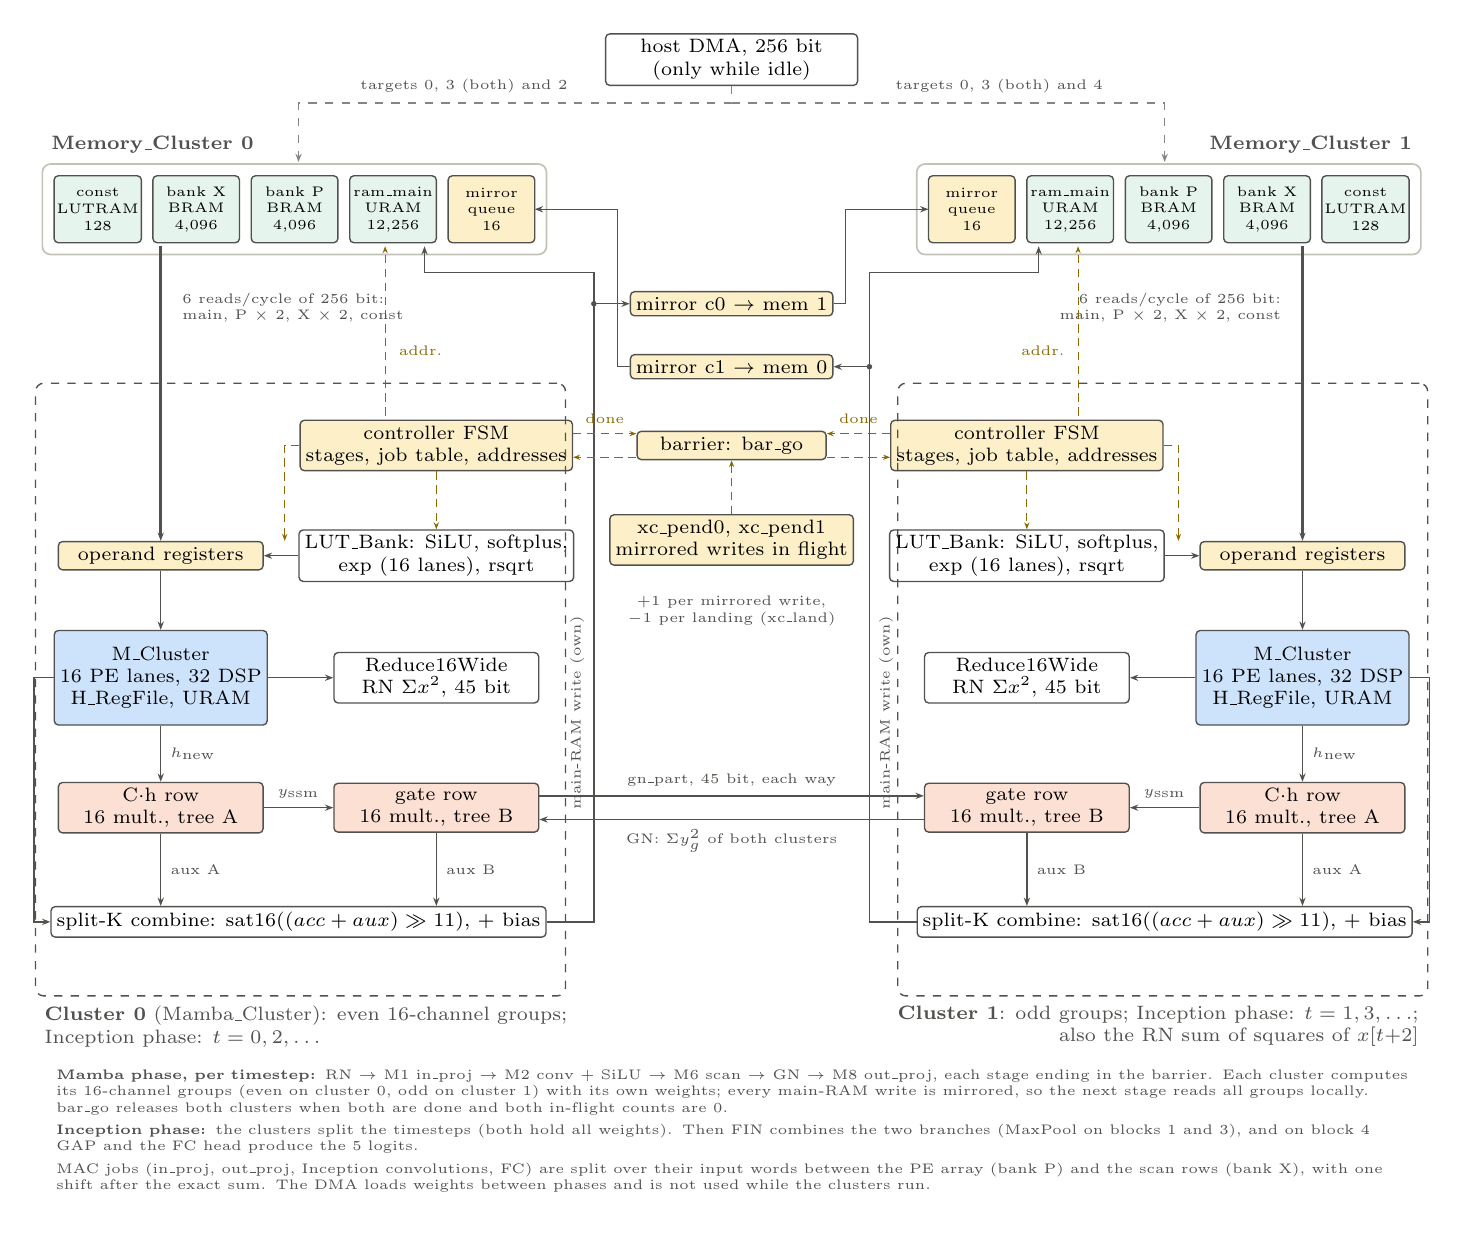
\begin{tikzpicture}[x=1cm,y=1cm]
  % ================================================================ host DMA
  \node[plain, minimum width=3.2cm] (dma) at (9.0,15.3) {host DMA, 256 bit\\(only while idle)};
  \draw[dma] (dma.south) -- (9.0,14.75) -| (3.5,14.0);
  \draw[dma] (9.0,14.75) -| (14.5,14.0);
  \node[tlbl, anchor=south] at (5.6,14.75) {targets 0, 3 (both) and 2};
  \node[tlbl, anchor=south] at (12.4,14.75) {targets 0, 3 (both) and 4};

  % ================================================================ memories
  \foreach \s/\sg in {0/1, 1/-1} {
    \begin{scope}[xshift={\s*18cm}, xscale=\sg]
      \node[mm] (const\s) at (0.95,13.4) {const\\LUTRAM\\128};
      \node[mm] (bx\s)    at (2.2,13.4)  {bank X\\BRAM\\4,096};
      \node[mm] (bp\s)    at (3.45,13.4) {bank P\\BRAM\\4,096};
      \node[mm] (main\s)  at (4.7,13.4)  {ram\_main\\URAM\\12,256};
      \node[mm, fill=fillCtl] (q\s) at (5.95,13.4) {mirror\\queue\\16};
    \end{scope}}
  \node[grp, fit={(const0) (q0)}] (mem0) {};
  \node[grp, fit={(const1) (q1)}] (mem1) {};
  \node[lbl, anchor=south west] at (mem0.north west) {\textbf{Memory\_Cluster 0}};
  \node[lbl, anchor=south east] at (mem1.north east) {\textbf{Memory\_Cluster 1}};

  % ================================================================ clusters
  \clusterbody{0}{1.75}{5.25}{3.5}
  \clusterbody{1}{16.25}{12.75}{14.5}
  \node[dgrp, fit={(0.3,11.05) (6.75,3.55)}] (cl0) {};
  \node[dgrp, fit={(11.25,11.05) (17.7,3.55)}] (cl1) {};
  \node[lbl, anchor=north west, align=left] at (cl0.south west) {\textbf{Cluster 0} (Mamba\_Cluster): even 16-channel groups;\\Inception phase: $t = 0, 2, \ldots$};
  \node[lbl, anchor=north east, align=right] at (cl1.south east) {\textbf{Cluster 1}: odd groups; Inception phase: $t = 1, 3, \ldots$;\\also the RN sum of squares of $x[t{+}2]$};

  % reads, addresses, own writes
  \foreach \s/\xo/\xa in {0/1.75/4.6, 1/16.25/13.4} {
    \draw[arr, line width=0.9pt] (\xo,12.93) -- (opr\s.north);
    \draw[carr] (\xa,10.78) -- (\xa,12.93);}
  \draw[arr] (cmb0.east) -- (7.25,4.35) -- (7.25,12.6) -- (5.1,12.6) -- (5.1,12.93);
  \draw[arr] (cmb1.west) -- (10.75,4.35) -- (10.75,12.6) -- (12.9,12.6) -- (12.9,12.93);
  \node[tlbl, anchor=west, align=left] at (1.9,12.15) {6 reads/cycle of 256 bit:\\main, P $\times$ 2, X $\times$ 2, const};
  \node[tlbl, anchor=east, align=right] at (16.1,12.15) {6 reads/cycle of 256 bit:\\main, P $\times$ 2, X $\times$ 2, const};
  \node[clbl, anchor=west] at (4.65,11.6) {addr.};
  \node[clbl, anchor=east] at (13.35,11.6) {addr.};
  \node[tlbl, anchor=south, rotate=90] at (7.25,7.0) {main-RAM write (own)};
  \node[tlbl, anchor=north, rotate=90] at (10.75,7.0) {main-RAM write (own)};
  % acc_raw into the combine
  \draw[arr] (mcl0.west) -- ++(-0.25,0) |- ($(cmb0.west)+(0,0)$);
  \draw[arr] (mcl1.east) -- ++(0.25,0) |- (cmb1.east);

  % ================================================================ mirrored writes
  \node[ctl, minimum width=2.1cm] (d0) at (9.0,12.2) {mirror c0 $\to$ mem 1};
  \node[ctl, minimum width=2.1cm] (d1) at (9.0,11.4) {mirror c1 $\to$ mem 0};
  \draw[arr] (7.25,12.2) -- (d0.west);
  \draw[arr] (d0.east) -- (10.45,12.2) -- (10.45,13.4) -- (11.5,13.4);
  \draw[arr] (10.75,11.4) -- (d1.east);
  \draw[arr] (d1.west) -- (7.55,11.4) -- (7.55,13.4) -- (6.5,13.4);
  \fill[inkB] (7.25,12.2) circle (0.035) (10.75,11.4) circle (0.035);

  % ================================================================ barrier
  \node[ctl, minimum width=2.4cm] (cnt) at (9.0,9.2) {xc\_pend0, xc\_pend1\\mirrored writes in flight};
  \node[ctl, minimum width=2.4cm] (bar) at (9.0,10.4) {barrier: bar\_go};
  \draw[carr] (cnt) -- (bar);
  \draw[carr] ($(fsm0.east)+(0,0.15)$) -- ($(bar.west)+(0,0.15)$) node[clbl, pos=0.5, above] {done};
  \draw[carr] ($(bar.west)+(0,-0.15)$) -- ($(fsm0.east)+(0,-0.15)$);
  \draw[carr] ($(fsm1.west)+(0,0.15)$) -- ($(bar.east)+(0,0.15)$) node[clbl, pos=0.5, above] {done};
  \draw[carr] ($(bar.east)+(0,-0.15)$) -- ($(fsm1.west)+(0,-0.15)$);
  \node[tlbl, align=center] at (9.0,8.3) {$+1$ per mirrored write,\\$-1$ per landing (xc\_land)};

  % ================================================================ GN exchange
  \draw[arr] ($(gtb0.east)+(0,0.15)$) -- ($(gtb1.west)+(0,0.15)$);
  \draw[arr] ($(gtb1.west)+(0,-0.15)$) -- ($(gtb0.east)+(0,-0.15)$);
  \node[tlbl, anchor=south] at (9.0,5.95) {gn\_part, 45 bit, each way};
  \node[tlbl, anchor=north] at (9.0,5.65) {GN: $\Sigma y_g^2$ of both clusters};

  % ================================================================ notes
  \node[tlbl, anchor=north west, align=left, text width=17.2cm] at (0.3,2.6) {%
    \textbf{Mamba phase, per timestep:} RN $\to$ M1 in\_proj $\to$ M2 conv + SiLU $\to$ M6 scan $\to$ GN $\to$ M8
    out\_proj, each stage ending in the barrier. Each cluster computes its 16-channel groups (even on cluster 0, odd
    on cluster 1) with its own weights; every main-RAM write is mirrored, so the next stage reads all groups
    locally. bar\_go releases both clusters when both are done and both in-flight counts are 0.\\[2pt]
    \textbf{Inception phase:} the clusters split the timesteps (both hold all weights). Then FIN combines the two
    branches (MaxPool on blocks 1 and 3), and on block 4 GAP and the FC head produce the 5 logits.\\[2pt]
    MAC jobs (in\_proj, out\_proj, Inception convolutions, FC) are split over their input words between the PE array
    (bank P) and the scan rows (bank X), with one shift after the exact sum. The DMA loads weights between phases
    and is not used while the clusters run.};
\end{tikzpicture}
\end{document}
